\chapter{Mise en œuvre et résultats} 

\lettrine{M}{aintenant} que le modèle est posé et que l'on sait quelles méthodes utiliser pour la calibration et le choix des solutions, on peut calibrer le modèle et présenter et explorer les solutions optimales.

\section{Solutions pour le modèle initial}

On présente dans cette section des solutions pour le modèle initial, avant de tester d'autres hypothèses.

\subsubsection{Analyse de sensibilité}

La première étape à effectuer est l'analyse de sensibilité.
Il faut cependant au préalable définir les intervalles dans lesquels évoluent nos paramètres.
Si pour certains paramètres, les intervalles semblent naturels à choisir comme l'intervalle $[0; 1]$ pour les probabilités, le choix d'intervalles pour certains paramètres comme $\gamma$ s'avère plus délicat.
Procédons paramètre par paramètre.

En premier lieu, le paramètre $\gamma$ qui, rappelons-le, correspond au coefficient de proportionnalité sur les inflorescences vivantes qui permet de déterminer le nombre de femelles exogènes arrivant dans chaque sous-parcelle à chaque date.
Ce paramètre est propre à notre modèle, on ne peut donc pas trouver d'estimation dans la littérature.
On peut fixer la borne inférieure de l'intervalle à 0, en partant du principe qu'une cécidomyie préfère rester dans le verger duquel elle émerge plutôt que de migrer dans un autre verger.
On fixera la borne supérieure à 1. Cela signifie qu'il ne peut pas y avoir plus de femelles exogènes qui arrivent dans le verger que ce qu'il n'y a d'inflorescences.

Ensuite, par définition du paramètre $p_{\text{m}}$ (qui régule les échanges de femelles entre les trois sous-parcelles), on sait qu'il évolue dans l'intervalle $[0;1]$.
De la même manière, $\mu_{\text{ER}}$ et $\mu_{\text{EH}}$ désignent les probabilités de survie aux modalités de couverture du sol ER et EH.
Leurs intervalles seront donc aussi $[0;1]$.

Le paramètre $k$ relatif à la disponibilité en ressources gère le nombre d'attaques de cécidomyies que peut subir une inflorescence chaque jour sans qu'il n'y ait de compétition pour la ressource.
En l'absence d'estimation ou de référence sur la valeur de ce paramètre, il sera fixé de manière assez large en 0.01 et 10.

Le \texttt{stock} d'individus en diapause sera fixé de manière assez large, dû à une absence d'estimation, entre 500 et 20000.

Enfin, le nombre d'œufs pondus qui survivent $E_0\mu_\ell$ est présent dans la littérature \citep{paul}.
Sa valeur est de 6, mais nous paraît peu fiable.
On le calibrera autour de cette valeur, entre 1 et 11.

Les intervalles étant définis, on peut maintenant faire l'analyse de sensibilité. Les résultats, pour un échantillon de taille $N = 50000$, sont visibles sur la figure~\ref{fig:sa}.

\begin{figure}
 \centering
 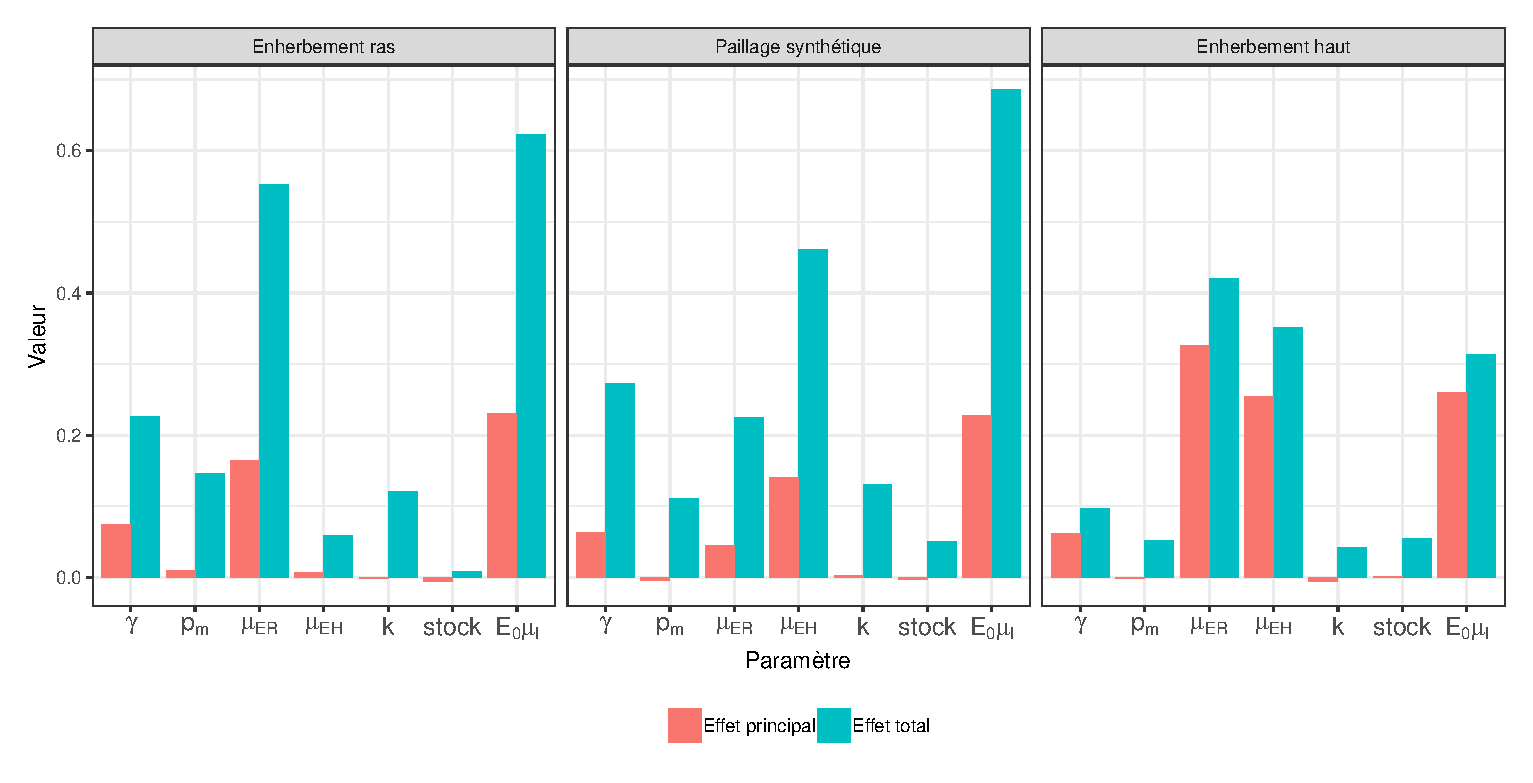
\epsfig{file = plots/sensitivity_analysis_A.eps, scale = 0.59}
 \caption{Analyse de sensibilité de notre modèle avec la méthode Sobol.}
 \label{fig:sa}
\end{figure}

On obtient ainsi les effets principaux et les effets totaux de Sobol pour chaque sous-parcelle.

Pour l'enherbement ras, le paramètre qui induit le plus de variance (effet principal) est $E_0\mu_\ell$ qui donne le nombre d'œufs arrivant au troisième stade de développement larvaire.
Sans surprise le probabilité de survie à la modalité de couverture du sol ER apporte aussi beaucoup de variance à cette sous-parcelle.
Ensuite, l'apport en variance du paramètre $\gamma$ n'est pas négligeable non plus.
En revanche, les quatre autres paramètres n'apportent en eux-même que peu de variance relativement aux trois autres nommés ci-dessus.
On remarque également que les paramètres qui apportent le plus de variance sont aussi ceux dont les interactions induisent le plus de variance.
(La variance apportée par les interactions d'un paramètre correspond à la différence entre l'effet total et l'effet principal).

Pour le paillage synthétique, c'est aussi $E_0\mu_\ell$ qui apporte le plus de variance.
Viennent ensuite $\mu_{\text{EH}}, \gamma$ et $\mu_{\text{ER}}$.
Les paramètres $p_{\text{m}}, k$ et \texttt{stock} n'apportent pas de variance.
Il est intéressant de noter que la probabilité de survie à la modalité de couverture du sol de la sous-parcelle EH a plus d'impact que celle de la sous-parcelle ER.
Ici aussi, ce sont les paramètres qui apportent le plus de variance qui ont le plus d'interactions.

Pour l'enherbement haut, c'est la probabilité de survie à la modalité de couverture du sol ER $\mu_{\text{ER}}$ qui apporte le plus de variance, ce qui est assez peu intuitif.
Il est suivi de près par deux autres paramètres : $\mu_{\text{EH}}$ et $E_0\mu_{\ell}$.
La part de variance apportée par le paramètre $\gamma$ n'est pas négligeable.
Celle apportée par $p_{\text{m}}, k$ et \texttt{stock} est négligeable.
Et une fois encore, ce sont les paramètres qui apportent le plus de variance qui ont le plus d'interactions.
% On s'aperçoit que le paramètre apportant le plus de variance à la sortie de notre modèle (effet principal) est $E_0\mu_\ell$, et ce pour chacune des trois sous-parcelles.
% Viennent ensuite les probabilités de survie à la modalité de couverture du sol.
% Sans surprise, le paramètre $\mu_{\text{EH}}$ apporte beaucoup de variance à la sous-parcelle avec la modalité de couverture de sol correspondante.
% De façon moins intuitive, ce paramètre apporte aussi beaucoup de variance à la sous-parcelle avec un enherbement haut.
% Il y apporte même plus de variance que le paramètre $\mu_{\text{EH}}$, bien que ce dernier en apporte aussi une part importante.
% Concernant la sous-parcelle avec un paillage synthétique, les probabilités de survie aux modalités de couverture du sol apporte aussi de la variance, avec un avantage pour $\mu_{\text{EH}}$.
% À noter que le paramètre $\gamma$ n'est pas en reste non plus, induisant une part non-négligeable de variance sur chacune des trois-sous-parcelles.
% Les paramètres $p_{\text{m}}, k$ et \texttt{stock} n'apportent en eux-mêmes que peu de variance.
% 
% On remarque également que les paramètres qui apportent le plus de variance sont aussi ceux dont les interactions induisent le plus de variance. (La variance apportée par les interactions d'un paramètre correspond à la différence entre l'effet total et l'effet principal).

Certains de ces résultats ne sont pas surprenants.
Il faut notamment se rappeler que le modèle est évalué sur l'estimation du nombre de larves, et que $E_0\mu_\ell$ intervient dans l'équation du modèle donnant le nombre de larves.
Ainsi, ce paramètre seul --- à valeur entre 1 et 11 --- peut facilement doubler le nombre de larves en fonction de sa valeur. Et induit donc naturellement une forte variance dans le modèle.
Et ce paramètre n'est interprétable que si l'on considère la valeur des autres paramètres.
Car un nombre élevé d'œufs pondus qui survivent peut être compensé par une faible probabilité de survie aux modalités de couverture de sol et une faible arrivée d'individus exogènes --- et vice-versa.
Ce qui peut expliquer ses fortes interactions.
Cette analyse de sensibilité montre surtout l'impact des probabilités de survie aux modalités de couverture du sol en fonction de chaque sous-parcelles, qui ne respecte pas ce que l'on pourrait s'imaginer \emph{a priori}.
On retiendra également que trois de nos paramètres ($p_{\text{m}}, k$ et \texttt{stock}) n'ont qu'un impact très limité --- comparativement aux autres --- sur la sortie du modèle.

\subsection{Calibration et choix des solutions}

En utilisant les mêmes intervalles pour les paramètres que ceux utilisés par l'analyse de sensibilité, on peut utiliser NSGA-II.
% pour obtenir un sous-ensemble du front de Pareto contenant des jeux de paramètres produisant des solutions non-dominées.
% L'algorithme est cependant stochastique, il ne renvoie jamais exactement deux fois les mêmes résultats.
% Pour pallier cet aspect, on exécute trente fois la fonction \texttt{nsga2} \citep{nsga} (avec une taille de population de 200, et 200 générations).
% Cela nous donne ainsi 6000 solutions. Mais parmi ces 6000 solutions certaines sont peut-être dominées par d'autres solutions provenant d'une exécution de \texttt{nsga2} différente.
% On ne récupère alors que les solutions non-dominées (et les jeux de paramètres correspondants) grâce à la fonction \texttt{is\textunderscore dominated} \citep{emoa}.
% Après avoir exécuté trente fois la fonction \texttt{nsga2} \citep{nsga} suivie de la fonction \texttt{is\textunderscore dominated} \citep{emoa} pour récupérer les solutions non-dominées.
% 
% on obtient ainsi 842 jeux de paramètres produisant autant de solutions non-dominées, parmi lesquelles on peut sélectionner des solutions.
% \subsection{Choix de solutions}
% On peut maintenant essayer de repérer différentes solutions--types reproduisant les quantités de larves observées.
% On effectue une CAH avec l'indice de Ward en utilisant la fonction \texttt{hclust} \citep{R}.
Parmi les 6000 solutions générées par la calibration du modèle avec l'algorithme d'optimisation NSGA-II, on a obtenu 842 jeux de paramètres produisant des solutions non-dominées.
Pour repérer par CAH les différentes solutions types parmi ces 842 solutions non-dominées, il faut dans un premier temps choisir un nombre de classes.
À cette fin, on regarde l'inertie intra-classes en fonction du nombre de classes (voir figure~\ref{fig:caha}).
Dans une optique de classification «classique», choisir 2, 3, 6 ou 8 classes pourrait s'avérer pertinent.
(Ces nombres de classes produisant une minimisation relativement importante de l'inertie intra-classes.)
Nous préférons cependant ne pas risquer de passer à côté d'une catégorie de solution potentiellement intéressante.
Nous choisirons 16 classes.

\begin{figure}[ht]
 \centering
 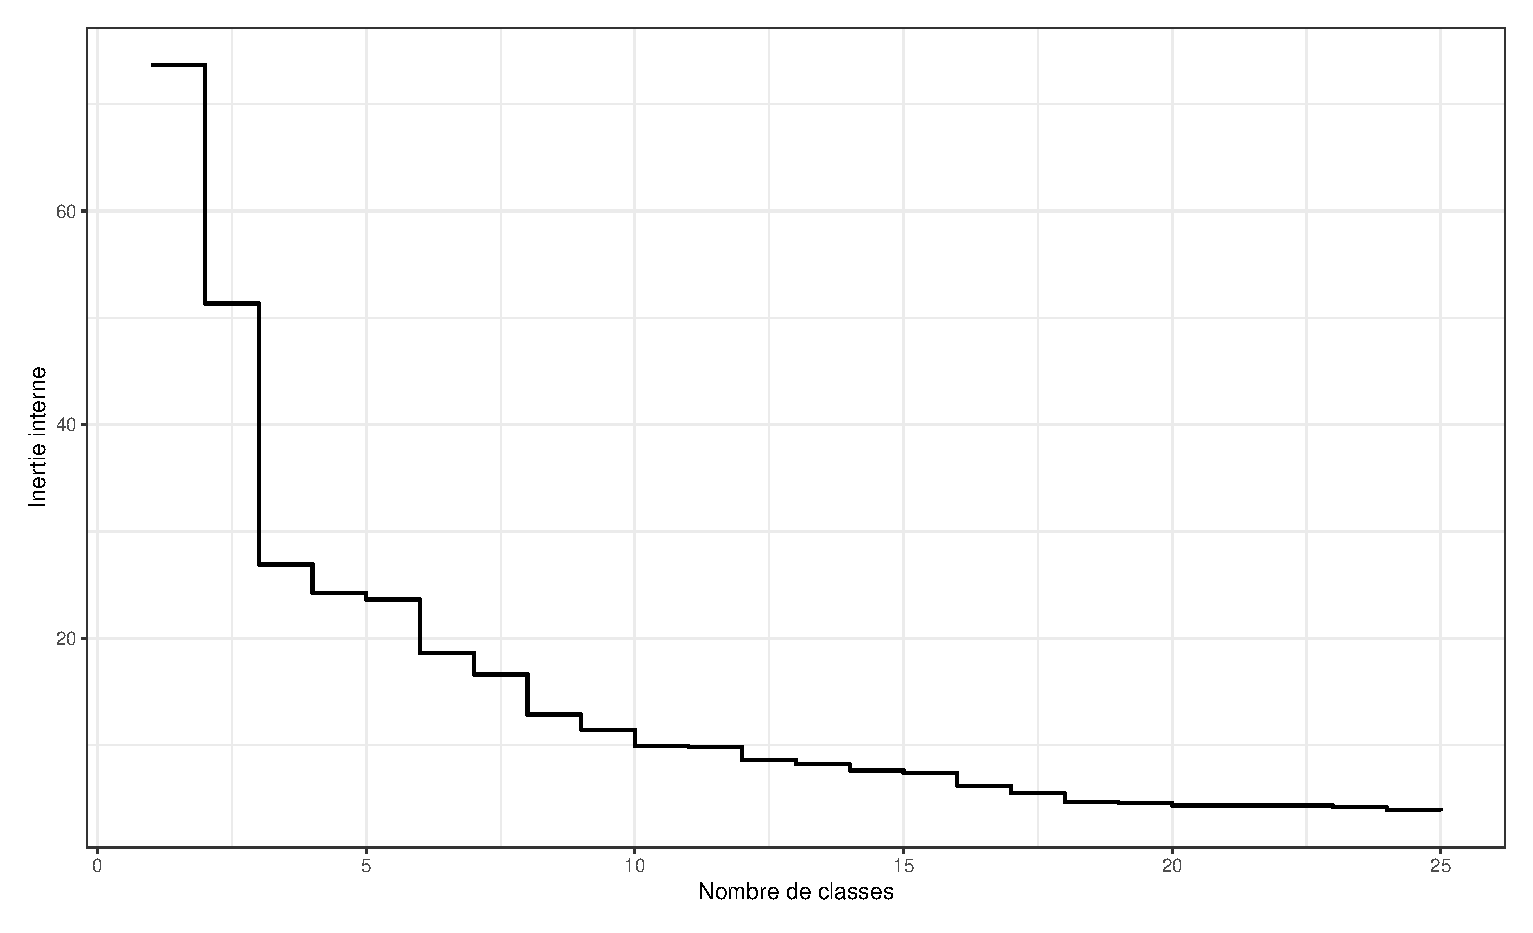
\epsfig{file = plots/cah_A.eps, scale = 0.55}
 \caption{Inertie intra-classes en fonction du nombres de classe obtenue par une CAH sur les jeux de paramètres renvoyés par NSGA-II.}
 \label{fig:caha}
\end{figure}


Parmi les 16 classes, trois solutions--types se distinguent.
Les solutions sont visibles sur la figure~\ref{fig:A1}.
On peut voir sur la figure la décomposition du nombre de larves en fonction de la provenance des femelles qui ont pondus les œufs.
Par exemple, si l'aire sous la courbe est essentiellement rouge, alors cela voudrait dire qu'il y a une forte proportion de femelles exogènes.
Et si elle est principalement verte, cela veut dire que la majorité des femelles qui pondent sont des femelles qui ont émergées dans une autre sous-parcelle. 
Cela peut questionner la pertinence biologique de la solution proposée, indépendamment de la qualité d'ajustement de la dynamique.

On détaille les trois solutions--types :
\begin{itemize}
 \item \textbf{Solution--type 1 :} 
 Les dynamiques pour les trois sous-parcelles sont grossièrement captées.
 Le modèle permet de simuler la présence plus précoce de cécidomyies sur la sous-parcelle ER et plus tardive sur les sous-parcelles PS et EH. 
 Il simule également un plus faible nombre de cécidomyies sur la sous-parcelle PS.
 Cependant le double pic caractérisant la dynamique des cécidomyies sur ER n'est pas capté, et la forte décroissance du nombre de cécidomyies en fin de saison est mal simulé.
 
 Les paramètres associées à ces trois dynamiques sont :
 \begin{center}
\begin{tabular}{lllllll}
$\gamma$ & $p_{\text{m}}$ & $\mu_{\text{ER}}$ & $\mu_{\text{EH}}$ & $k$ & \texttt{stock} & $E_0\mu_{\ell}$\\
0.08 & 0.494 & 0.976 & 0.046 & 1.928 & 5600 & 3.084
 \end{tabular}
 \end{center}
 Pour cette solution-type, on observe une quantité non négligeable de larves pondus par des femelles exogène (aire rouge), ce qui d'un point de vue biologique parait discutable.
L'absence d'individus qui émergent de la sous-parcelle EH s'explique par $\mu_{\text{EH}}$ qui est fixé à 0.046, ce qui veut dire que 95\% des larves meurent en essayant de s'enfouir dans la sous-parcelle ainsi que 95\% des femelles issues de pupaison ou de diapause qui essayent d'en émerger.
À la différence de la sous-parcelle ER où il n'y a pratiquement aucune mortalité induite par l'enherbement ras ($\mu_{\text{ER}} = 0.976$).
La valeur 0.8 attribuée à $\gamma$ est élevée (chose qui se confirmera empiriquement par les simulations qui suivront et qui peut déjà se voir sur la figure~\ref{fig:A1}).

\item \textbf{Solution--type 2 :} La qualité d'ajustement des dynamiques est assez similaire à celle de la première solution-type. Seule la décroissance en fin de saison est un peu mieux captée. Cependant, contrairement à la solution précédente qui avait trop d'individus exogènes, cette solution n'en a pas du tout.
On remarque également que les dynamiques des sous-parcelles PS et EH se composent uniquement de larves provenant d'œufs pondus par des femelles issues de la sous-parcelle ER.

Les paramètres sont :
 \begin{center}
\begin{tabular}{lllllll}
$\gamma$ & $p_{\text{m}}$ & $\mu_{\text{ER}}$ & $\mu_{\text{EH}}$ & $k$ & \texttt{stock} & $E_0\mu_{\ell}$\\
0 & 0.968 & 1 & 0.025 & 0.1 & 14483 & 6.26
 \end{tabular}
 \end{center}
 Ici aussi, il y a une absence totale d'individus qui émergent de la sous-parcelle avec un enherbement haut ($\mu_{\text{EH}} = 0.025$).
 L'absence d'individus exogènes se compensent par un nombre d'œufs pondus plus élevé que précédemment (6.26 contre 3.08) et un stock de larves diapausantes significatif (\texttt{stock} $=14483$).
 
\item \textbf{Solution--type 3 :}
Contrairement aux deux premières solutions, il y a ici des femelles qui émergent de la sous-parcelle EH.
Il faut cependant reconnaître que les dynamiques sont très mal captées : les problèmes d'ajustement des dynamiques identifiés pour les deux précédentes solutions sont toujours présents, et la décroissance en fin de saison est encore moins bien captée.

Les paramètres sont :
 \begin{center}
\begin{tabular}{lllllll}
$\gamma$ & $p_{\text{m}}$ & $\mu_{\text{ER}}$ & $\mu_{\text{EH}}$ & $k$ & \texttt{stock} & $E_0\mu_{\ell}$\\
0.026 & 0.93 & 0.565 & 0.647 & 0.174 & 13823 & 4.818
 \end{tabular}
 \end{center}
On observe que l'émergence d'individus dans la sous-parcelle EH ($\mu_{\text{EH}} = 0.647$ contre 0 précédemment) a entraîné une baisse d'émergence des individus dans la sous-parcelle ER ($\mu_{\text{ER}} = 0.565$ contre 0.97 et 1 pour les deux solutions précédentes)
 
\end{itemize}



\begin{figure}[ht]
 \centering
 \textbf{Solution--type 1}
 
 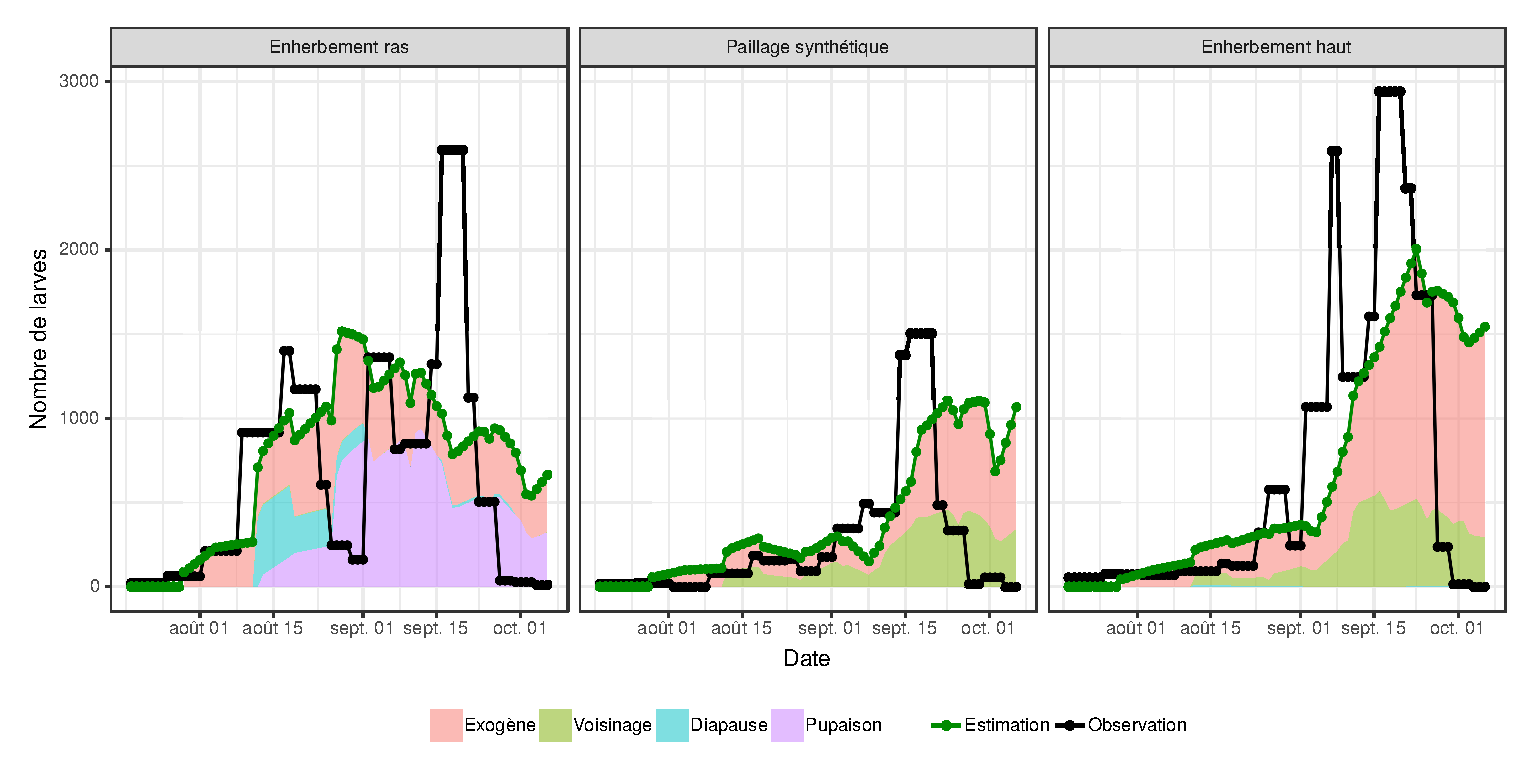
\epsfig{file = plots/A1.eps, scale = 0.52}
 
 \textbf{Solution--type 2}
 
 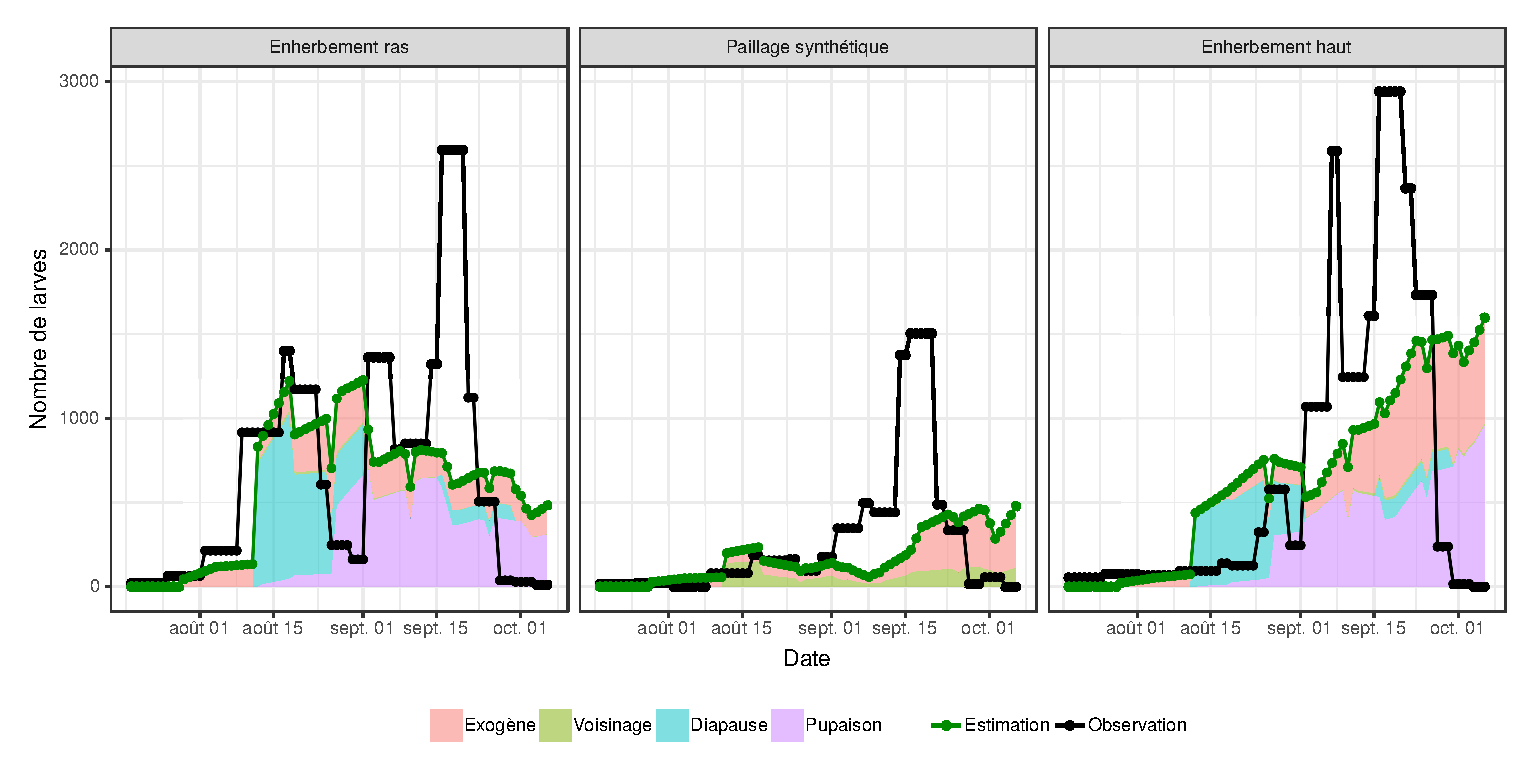
\epsfig{file = plots/A2.eps, scale = 0.52}
 
 \textbf{Solution--type 3}
 
 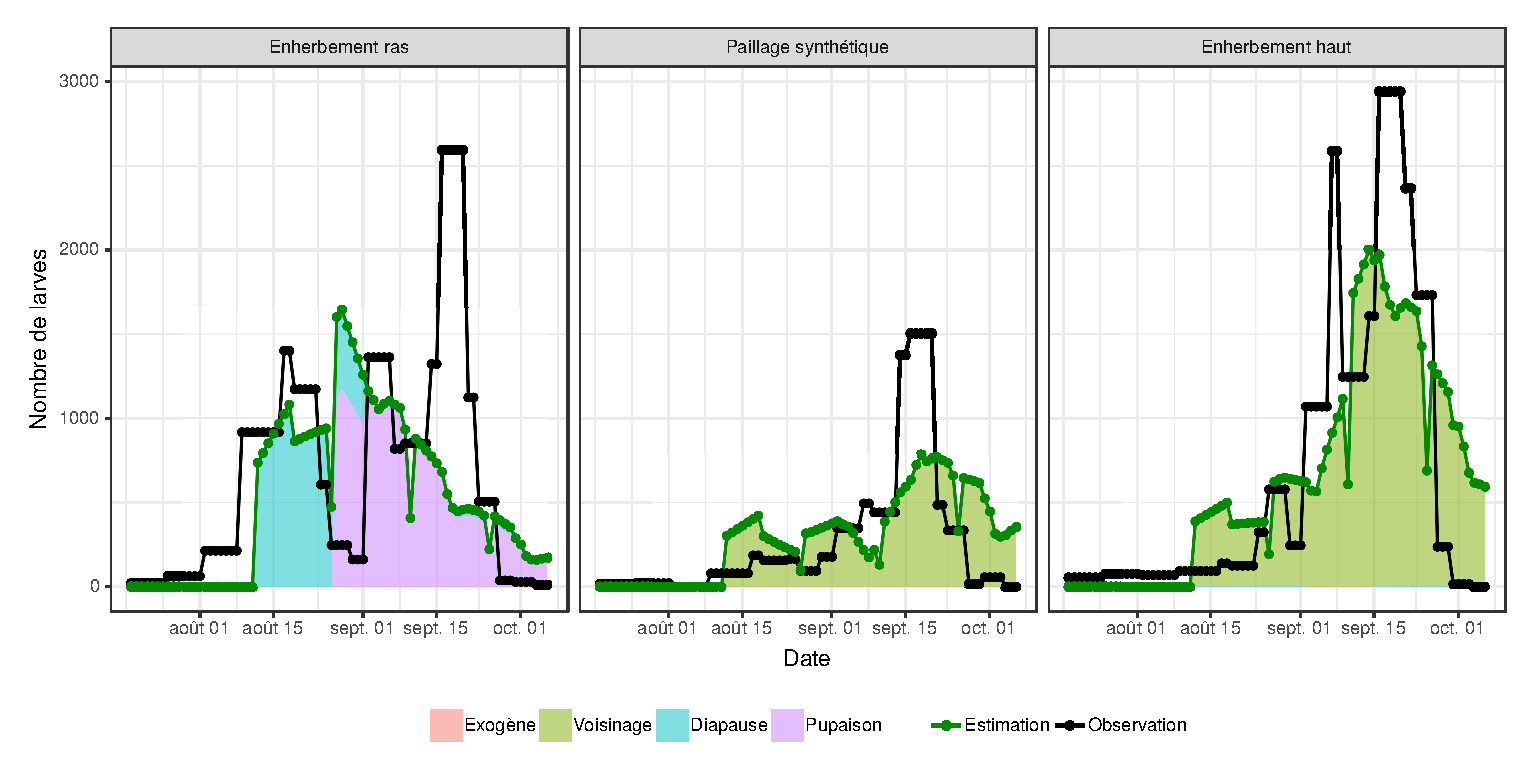
\epsfig{file = plots/A3.eps, scale = 0.52}
 \caption{Dynamiques observées et simulées pour chacune des trois solutions--types. La décomposition indiquant la provenance des femelles qui ont pondus les œufs est disponible pour les dynamiques simulées.}
 \label{fig:A1}
\end{figure}

Ces trois scénarios semblent tous montrer que le modèle actuel n'est pas suffisamment complet pour capter de façon satisfaisante le phénomène observé.
Pour les deux premières solutions, il y a quasiment aucun individus qui émergent de la sous-parcelle EH, et les individus se composent surtout d'individus exogènes (première solution-type) ou d'individus endogènes venant de la sous-parcelle ER (deuxième solution-type).
Et lorsqu'il y a des individus qui émergent de la sous-parcelle EH (troisième solution--type), le modèle ne parvient pas à recréer les dynamiques observées.

Cela peut s'expliquer par l'incapacité pour le modèle d'arrêter la reproduction des femelles et donc de stopper la dynamique en fin de saison induisant la baisse du nombre de larves observé.
C'est peut-être l'une des raisons pour laquelle le modèle fait appel  à beaucoup de femelles exogènes : elles sont proportionnelles aux inflorescences (dont la population baisse en fin de saison), ce qui entraîne donc une baisse du nombre de femelles et \emph{a fortiori} une baisse du nombre de larves.
Il y a dans le modèle un problème de décroissance en fin de saison.

Le modèle peut néanmoins être utilisé pour tester des hypothèses qui viendraient compléter ou remplacer les hypothèses initiales.
Et si en testant une de ces hypothèses, on trouve une solution qui permet d'ajuster convenablement les dynamiques et qui ne soit pas aberrante d'un point de vue biologique, on pourra alors essayer de valider la solution sur le verger n\textdegree2.


 
 \clearpage

\section{Solutions avec prise en compte de la température}

La première hypothèse à laquelle on s'intéresse est le lien entre la température et la probabilité d'entrer en pupaison.

On sait, d'après~\citet{pauldiap}, que la probabilité d'entrer en diapause et d'entrer en pupaison varie tout au long de l'année, et dépend de la température.
On espère ici qu'il y ait au cours de notre saison considérée (de juillet à octobre 2017) des variations de température pouvant expliquer une chute de la probabilité d'entrer en pupaison en fin de saison ce qui permettrait potentiellement au modèle de mieux reproduire la diminution du nombre de larves observées en fin de saison.

On choisira cependant la simplicité en essayant de trouver une relation linéaire permettant d'exprimer la probabilité d'entrer en pupaison en fonction de la température.
Pour réaliser ceci, on récupère les données de l'article de~\citet{pauldiap}.
Et à chaque taux de pupaison observé sur des larves prélevées en verger, on fait correspondre la température moyenne sur une quinzaine de jours (de 7 jours avant à 7 jours après la date du prélèvement).
On fait cela pour prendre en compte l'effet la température sur le cycle de développement complet de la cécidomyie --- depuis la ponte des œufs jusqu'à l'émergence des femelles issues de pupaison.


On effectue une régression linéaire simple de la probabilité d'entrer en pupaison en fonction de la température sur la quinzaine.
On fixera le seuil du risque de première espèce à $\alpha = 5\%$ pour le test de non-nullité des coefficients.
Les résultats sont visibles dans la table~\ref{tab:lm2}.

\begin{table}[hb]
\centering
\caption{Régression linéaire simple de la proportion d'individus en pupaison par la température moyenne sur 15 jours}
\label{tab:lm2}
\begin{tabular}{rrrrr}
 & Estimate & Std. Error & t value & Pr($>$$|$t$|$) \\ 
  \hline
(Intercept) & 1.9555 & 0.3665 & 5.34 & 0.0002 \\ 
  temp15j & -0.0550 & 0.0160 & -3.43 & 0.0050 \\ 
\end{tabular}
\end{table}

On en conclut que les coefficients associés à l'ordonnée à l'origine et à la température ne sont pas nuls et que l'on peut écrire
\[
p_{\text{p}} = 1.9555 - 0.055\times t_{15j}.
\]
La différence produite avec une probabilité constante fixée à 0.77, comme auparavant, est visible sur la figure~\ref{fig:pupaison}.
La différence en fin de saison est faible (environ 2\%), cela ne permettra pas \emph{a priori} d'améliorer le problème de la fin de saison.
En revanche, il y a des différences plus importantes au début de la saison de floraison qui pourraient peut-être améliorer l'ajustement général des dynamiques.

Les données utilisées proviennent d'observations effectuées en condition de laboratoire.
On laissera alors au modèle la possibilité d'amplifier la variation de la probabilité de pupaison afin de prendre en compte au mieux les conditions climatiques qu'il y aurait pu avoir sur le verger.
On peut faire ceci en utilisant la relation linéaire de la probabilité de pupaison en fonction de la température (donné ci-dessus par $p_{\text{p}}$) et un coefficient $\varpi\in [1;4]$ qui intervient comme suit :
\[
\widetilde p_{\text{p}} = \left( p_{\text{p}} - \overline{p_{\text{p}}} \right) \times \varpi + \overline{p_{\text{p}}},
\]
où $\widetilde p_{\text{p}}$ sera la probabilité d'entrer en pupaison et d'y survivre utilisée par le modèle et $\overline{p_{\text{p}}}$ la moyenne de la probabilité de pupaison.

\begin{figure}[ht]
 \centering
 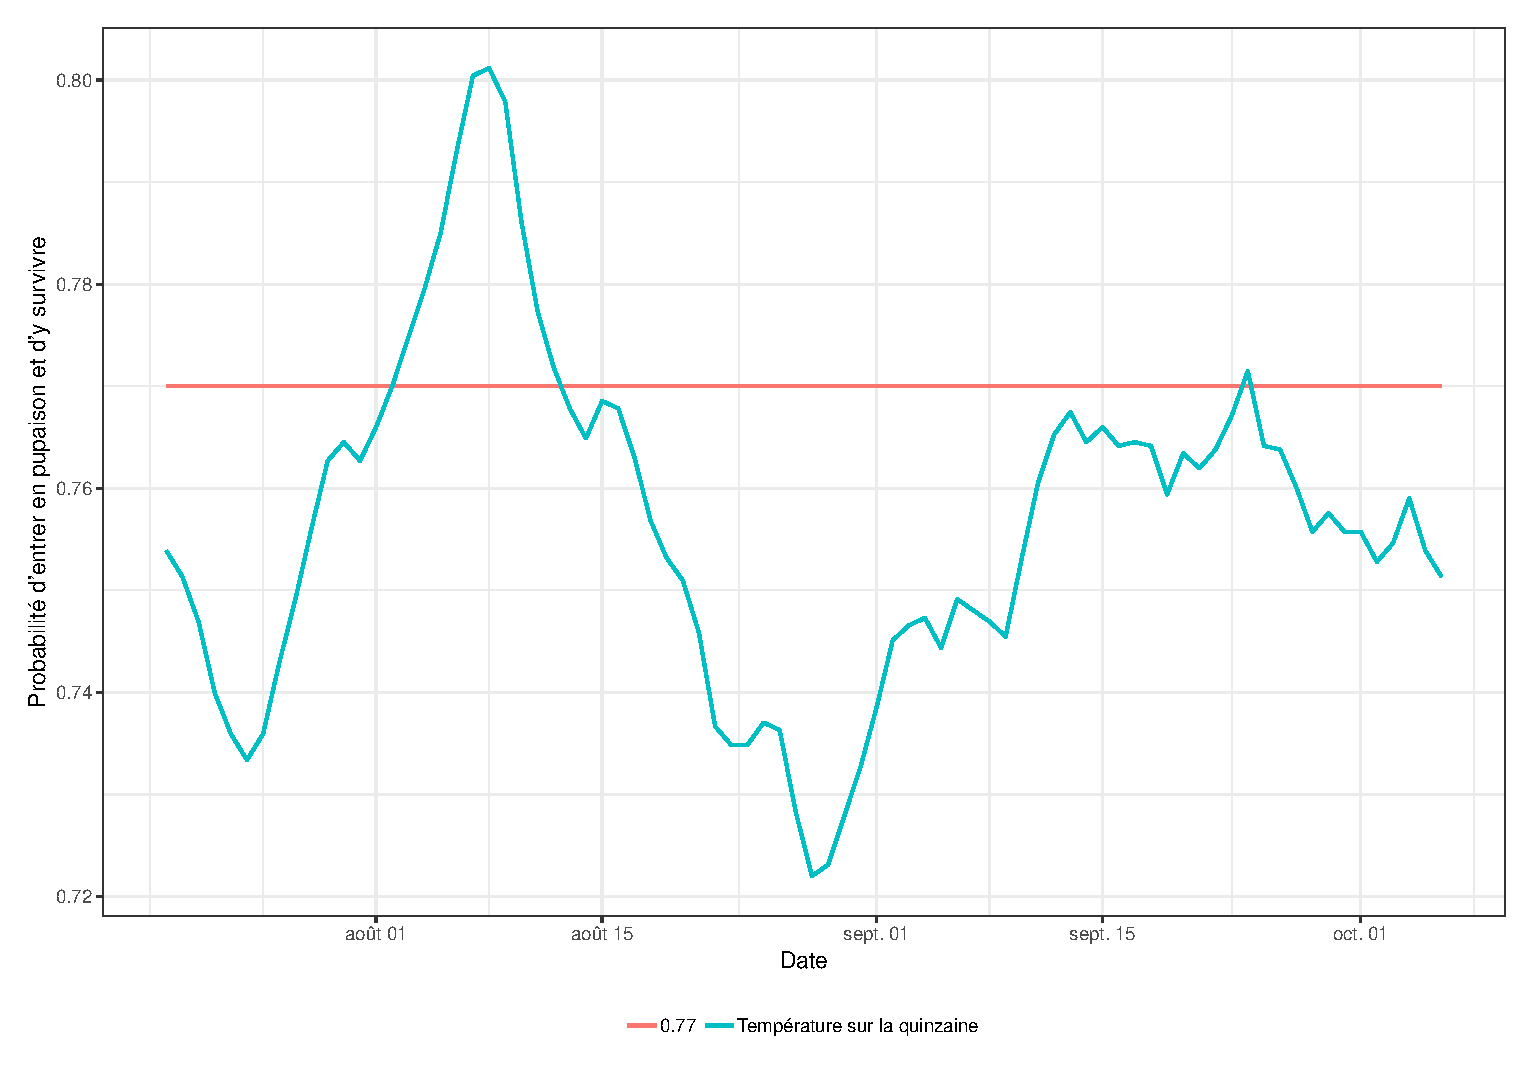
\epsfig{file = plots/pupaison.eps, scale = 0.55}
 \caption{Différence entre la probabilité d'entrer en pupaison et d'y survivre constante (égale à 0.77) et celle qui est fonction de la température moyenne sur la quinzaine.}
 \label{fig:pupaison}
\end{figure}
%

% Si l'on sait déjà que la température a un impact sur la sortie des individus en diapause, \citet{pauldiap} indique qu'elle a également un impact sur la probabilité d'entrer en pupaison.
% Intégrer cet aspect au modèle pourrait potentiellement permettre de réduire la reproduction de femelles endogènes en fin de saison, si la probabilité d'entrer en pupaison chute significativement.
% 
% On décide alors d'exprimer la probabilité d'entrer en pupaison et d'y survivre en fonction de la température.
% L'annexe~\ref{chap:pupaison} détaille la méthode utilisée.
% On se retrouve avec $p_{\text{p}}$ qui varie chaque jour et qui prend en compte la moyenne des températures quotidiennes sur quinze jours (de sept jours avant à sept jours après l'enfouissement).
% La différence produite avec une probabilité constante fixée à 0.77 est visible sur la figure~\ref{fig:pupaison}.
% 
% \begin{figure}[ht]
%  \centering
%  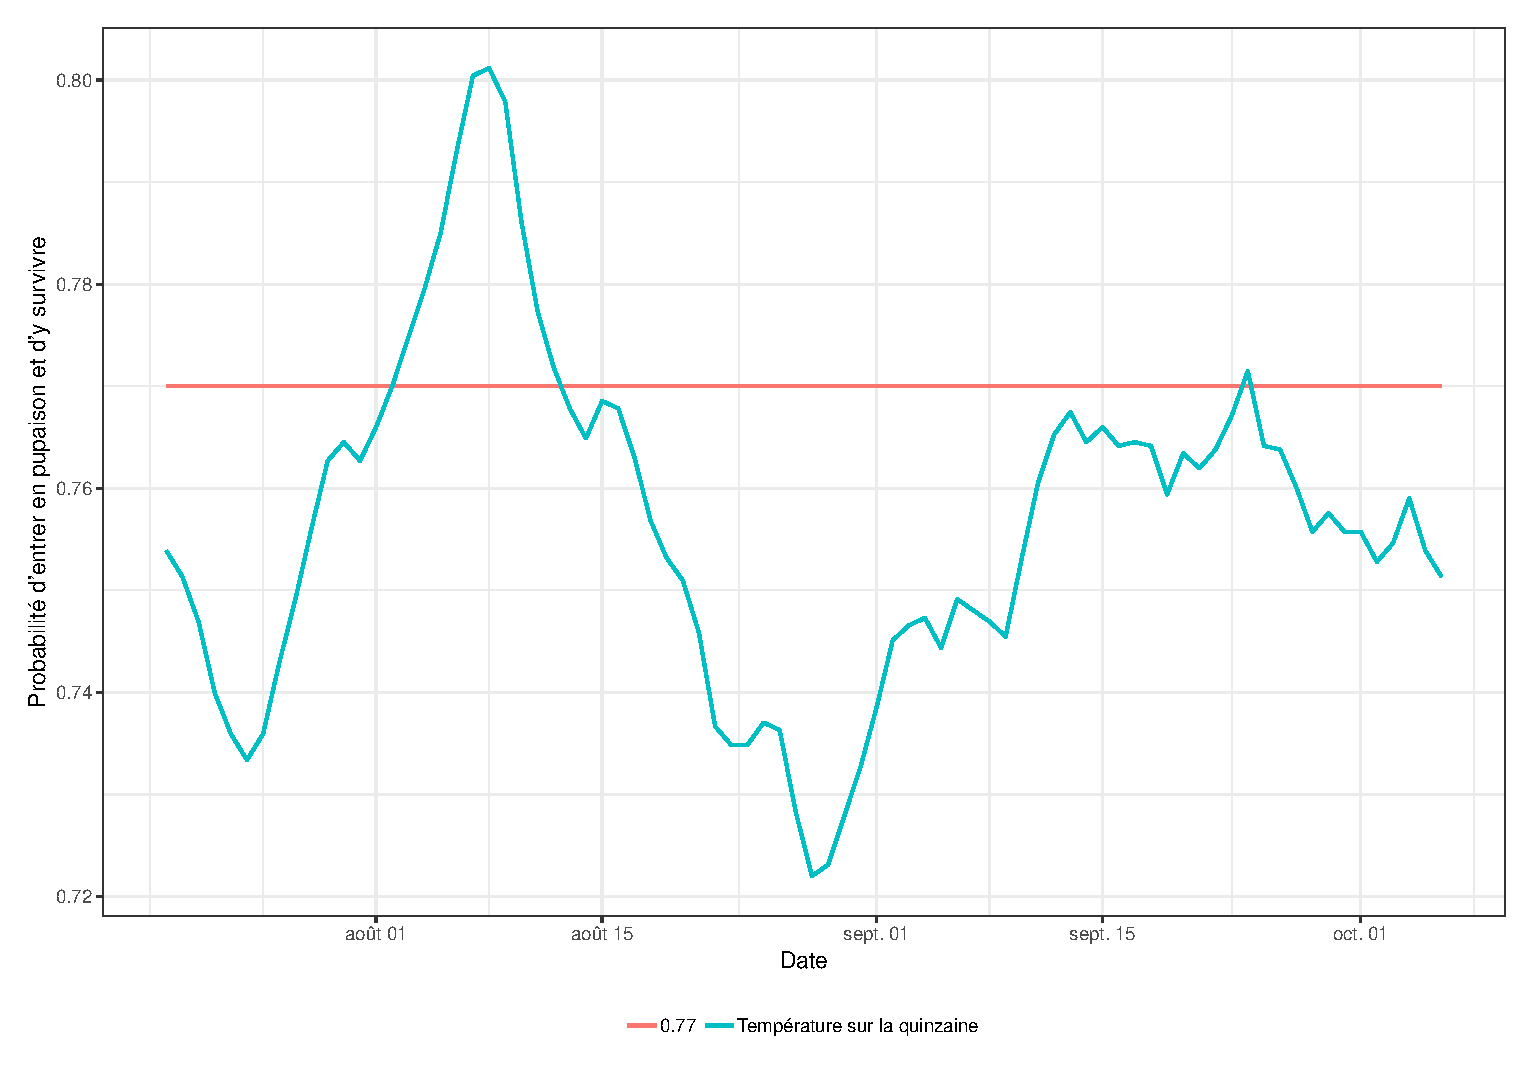
\epsfig{file = plots/pupaison.eps, scale = 0.55}
%  \caption{Différence entre la probabilité d'entrer en pupaison et d'y survivre constante (égale à 0.77) et celle qui est fonction de la température moyenne sur la quinzaine.}
%  \label{fig:pupaison}
% \end{figure}
% 
% On remarque peu de différences, c'est d'autant plus vrai en fin de saison où les deux probabilités sont très proches.
% Ce n'est donc pas l'effet de la température sur la phase de pupaison qui peut expliquer la diminution du nombre de larves observé en fin de saison.
% 
% On peut s'en convaincre en recalibrant le modèle avec cette nouvelle probabilité variable.
% On permet même au modèle «d'amplifier» la variabilité de la probabilité de pupaison en lui laissant le choix d'un certain coefficient $\varpi \in [1; 4]$ qui intervient comme suit :
% \[
% \widetilde p_{\text{p}} = \left( p_{\text{p}} - \overline{p_{\text{p}}} \right) \times \varpi + \overline{p_{\text{p}}},
% \]
% où $\widetilde p_{\text{p}}$ sera la probabilité d'entrer en pupaison et d'y survivre utilisée par le modèle.
% 
% Après obtention des résultats, on retrouve nos trois scénarios déjà présent dans la première version du modèle (voir figure~\ref{fig:B}).
% On peut noter que la calibration ne renvoie pas de valeur de $\varpi$ supérieure à 1.5, montrant que des variations dans la probabilité de rentrer en pupaison n'aide pas à améliorer l'ajustement des dynamiques.

Après calibration du modèle et classification des solutions, on trouve trois solutions--types, qui sont très similaires à celles trouvées avec le modèle initial.
Les voici :
\begin{itemize}
 \item \textbf{Solution--type 1 :} 
 Une solution faisant appel à beaucoup d'individus exogènes et sans individus qui émergent de la sous-parcelle EH.
 
 Les paramètres sont :
 \begin{center}
\begin{tabular}{llllllll}
$\gamma$ & $p_{\text{m}}$ & $\mu_{\text{ER}}$ & $\mu_{\text{EH}}$ & $k$ & \texttt{stock} & $E_0\mu_{\ell}$ & $\varpi$\\
0.044 & 0.715 & 0.998 & 0.002 & 0.143 & 1548 & 4.202 & 1.167
 \end{tabular}
 \end{center}

\item \textbf{Solution--type 2 :} 
Une solution sans individus exogènes ni sans individus qui émergent de la sous-parcelle EH  et sans individus exogènes.

Les paramètres sont :
 \begin{center}
\begin{tabular}{llllllll}
$\gamma$ & $p_{\text{m}}$ & $\mu_{\text{ER}}$ & $\mu_{\text{EH}}$ & $k$ & \texttt{stock} & $E_0\mu_{\ell}$ & $\varpi$\\
0 & 1 & 1 & 0.001 & 0.1 & 17188 & 6.3 & 1.036
 \end{tabular}
 \end{center}
 
\item \textbf{Solution--type 3 :}
Une solution avec des femelles qui émergent de la sous-parcelle EH.

Les paramètres sont :
 \begin{center}
\begin{tabular}{llllllll}
$\gamma$ & $p_{\text{m}}$ & $\mu_{\text{ER}}$ & $\mu_{\text{EH}}$ & $k$ & \texttt{stock} & $E_0\mu_{\ell}$ & $\varpi$\\
0.002 & 0.280 & 0.923 & 0.986 & 0.177 & 20066 & 3.288 & 1.110
 \end{tabular}
 \end{center}
\end{itemize}

Il n'est probablement pas très pertinent de s'étendre longuement sur ces trois nouvelles solutions, dans la mesure où elles sont très similaires aux solutions trouvées avec le modèle initial.
On peut remarquer que le paramètre $\varpi$ ne dépasse jamais 1.5, ce qui semble indiquer que la prise en compte de l'effet de la température sur la probabilité d'entrer en pupaison ne semble pas améliorer le modèle.

\begin{figure}[h]
 \centering
 \textbf{Solution--type 1}
 
 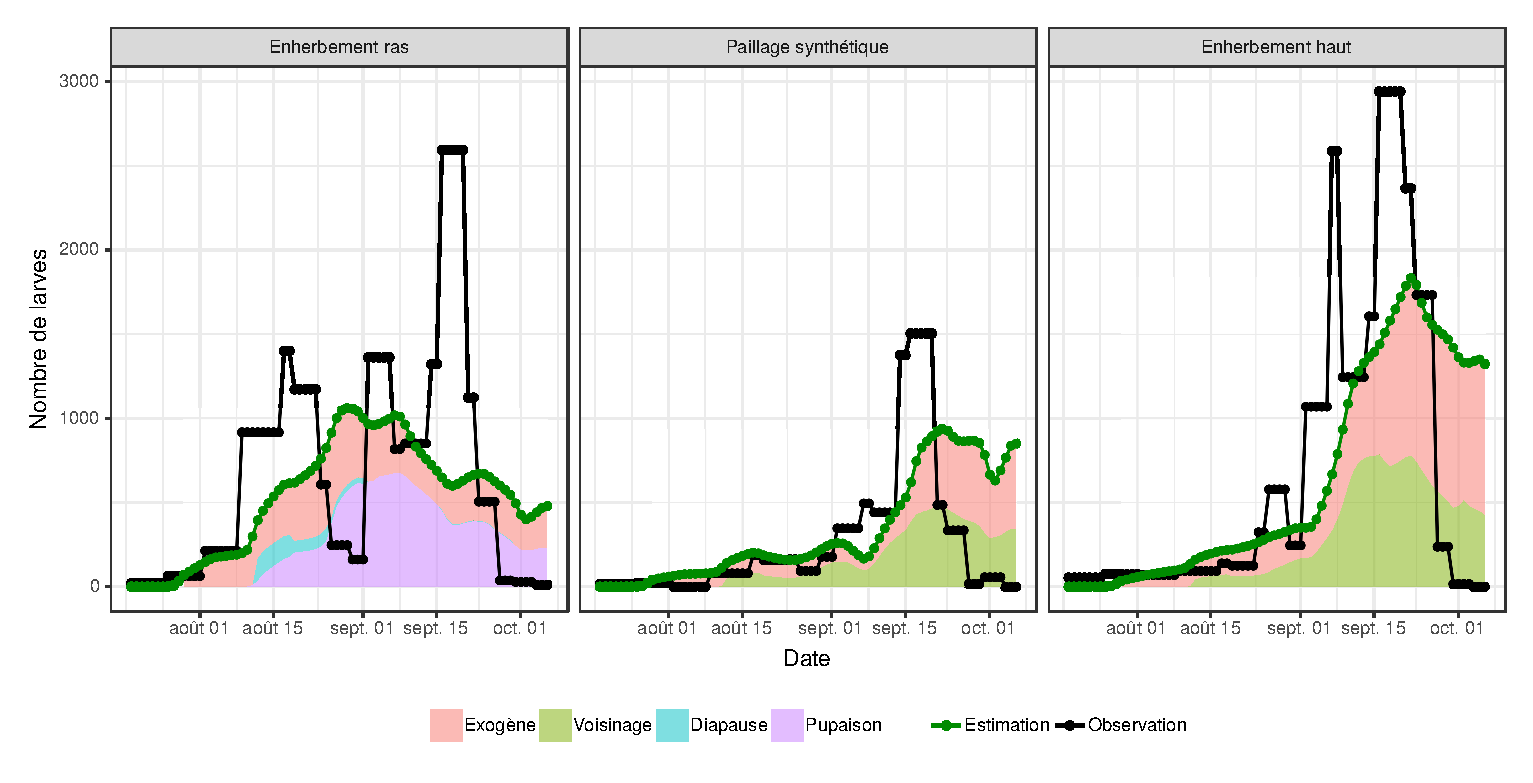
\epsfig{file = plots/B1.eps, scale = 0.52}
 
 \textbf{Solution--type 2}
 
 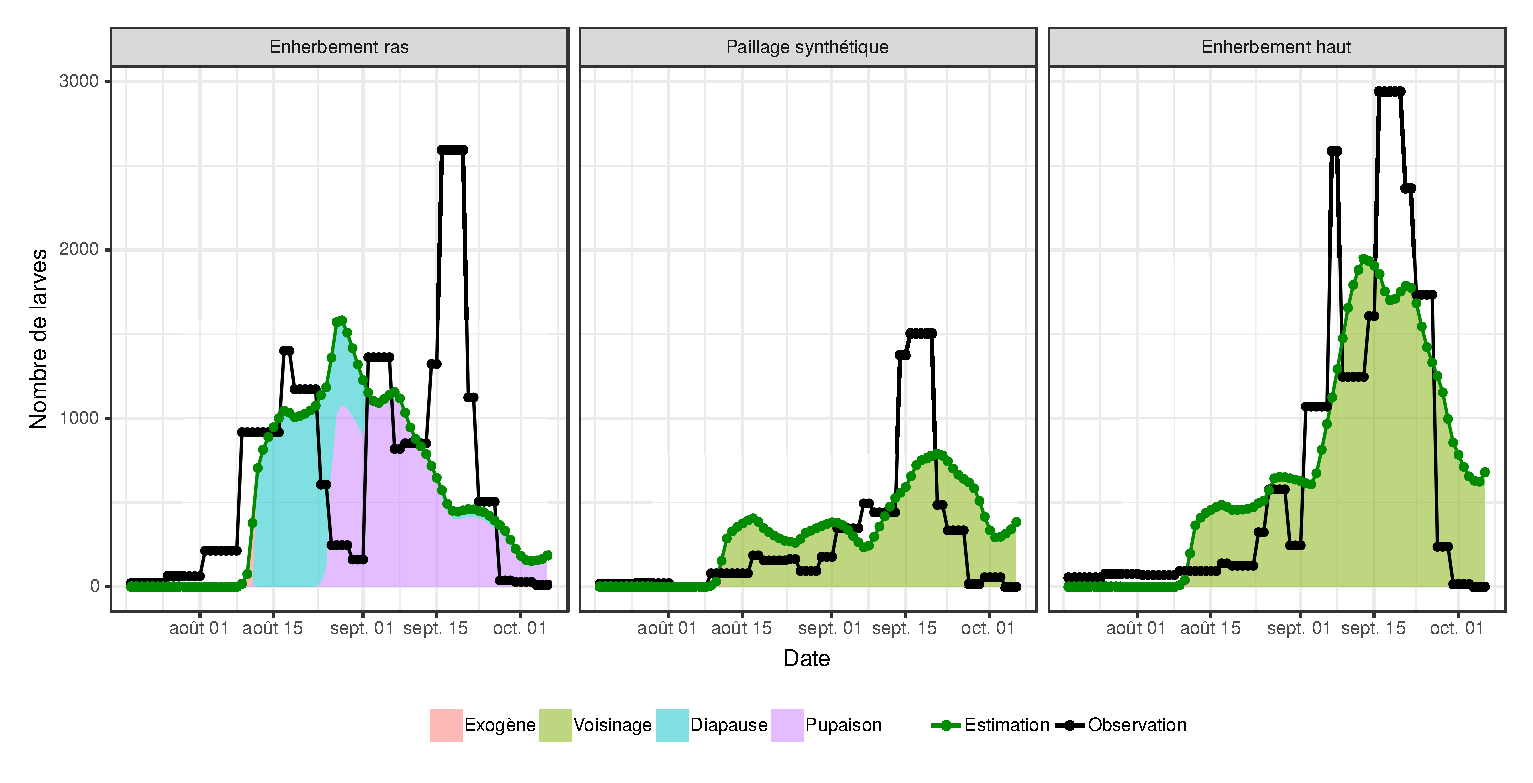
\epsfig{file = plots/B2.eps, scale = 0.52}
 
 \textbf{Solution--type 3}
 
 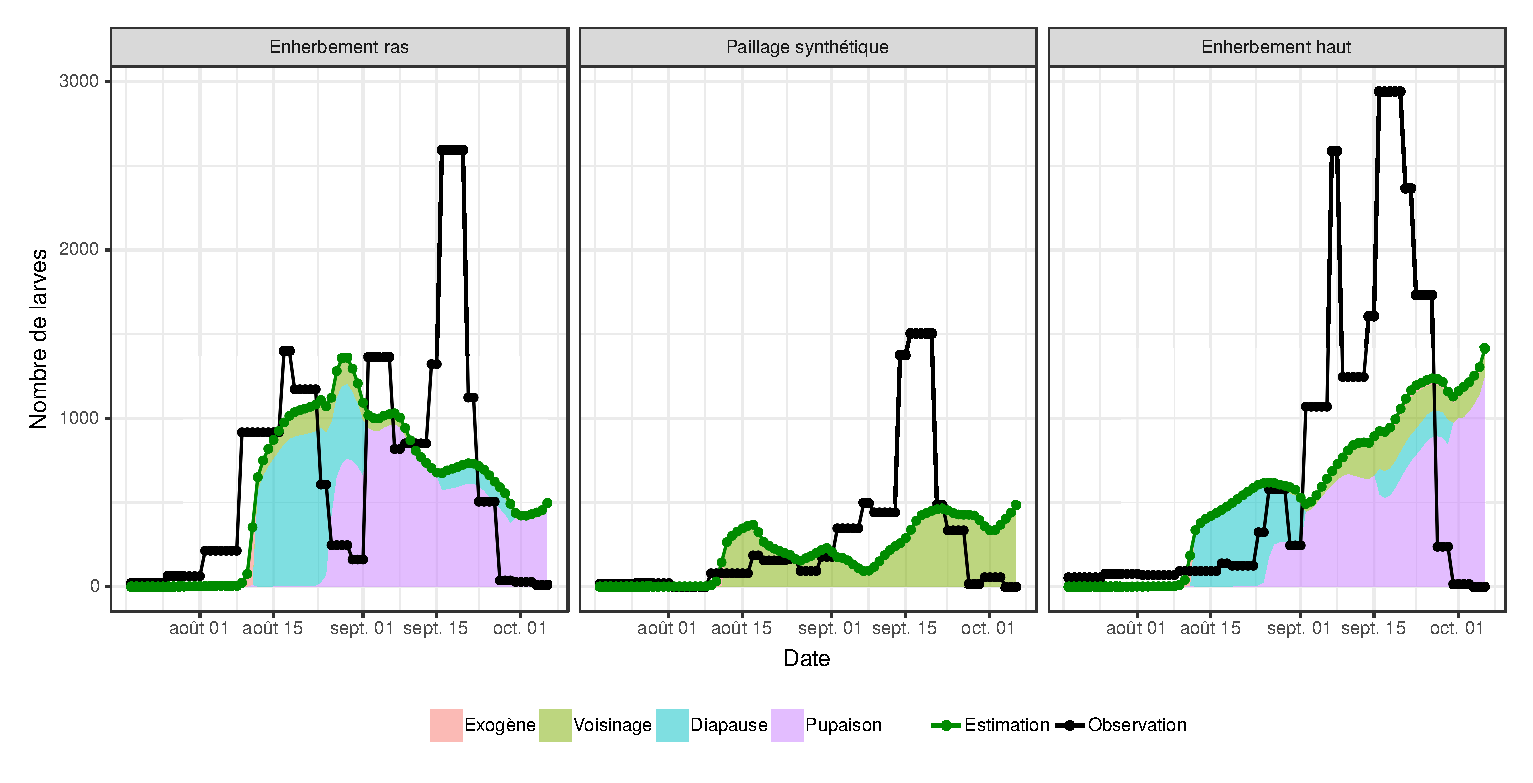
\epsfig{file = plots/B3.eps, scale = 0.52}
 \caption{Dynamiques observées et simulées pour chacune des trois solutions--types. La décomposition indiquant la provenance des femelles qui ont pondus les œufs est disponible pour les dynamiques simulées.}
 \label{fig:B}
\end{figure}

\clearpage
\section{Solutions avec prise en compte de contraintes liées aux ressources}

Puisque la température n'explique pas le phénomène observé en fin de saison, on teste une autre hypothèse.
On s'intéresse aux ressources.
L'intérêt pour les ressources est motivé par le fait que, sur les figures~\ref{fig:larves} et~\ref{fig:larves2}, les dynamiques de larves semblent corrélées avec les dynamiques d'inflorescences vivantes.
Les coefficients de corrélations de Spearman (du verger n\textdegree1) confirment plus ou moins cette intuition :
\[
\rho^{\text{ER}}\left( L_t, I_t  \right) =0.46,  \qquad \rho^{\text{PS}}\left( L_t, I_t  \right) =0.68, \qquad \rho^{\text{EH}}\left( L_t, I_t  \right) =0.76.
\]
On pourrait s'attendre à un décalage entre les dynamiques de larves et d'inflorescences, correspondant à la durée de développement qu'il faut entre la ponte et l'apparition du troisième stade larvaire.
Or, sur les figures~\ref{fig:larves} et~\ref{fig:larves2}, cela ne s'observe pas.

Pour expliquer cette absence de décalage, on émet une hypothèse.
Une inflorescence n'est pas attractive pour une cécidomyie de son débourrement jusqu'à la fin de sa vie mais uniquement lors des premiers stades phénologiques de l'inflorescence.
Lorsqu'elle atteint le stade phénologique F, la tige se durcit progressivement, rendant peut-être plus difficile la ponte pour les cécidomyies.
Notre hypothèse est que seules les inflorescences aux stades phénologiques C, D et E sont considérées comme attractives par les cécidomyies.

On détaille dans l'annexe~\ref{chap:deb} comment nous sommes capables de simuler des dynamiques d'inflorescences aux stades C, D et E.

Nous ferons ici l'hypothèse que la durée d'attractivité est de seize jours, ce qui correspond à la durée théorique des stades phénologiques C, D et E.
La différence entre les inflorescences vivantes et les inflorescences attractives est visible sur la figure~\ref{fig:CDE}.

\begin{figure}[ht]
 \centering
 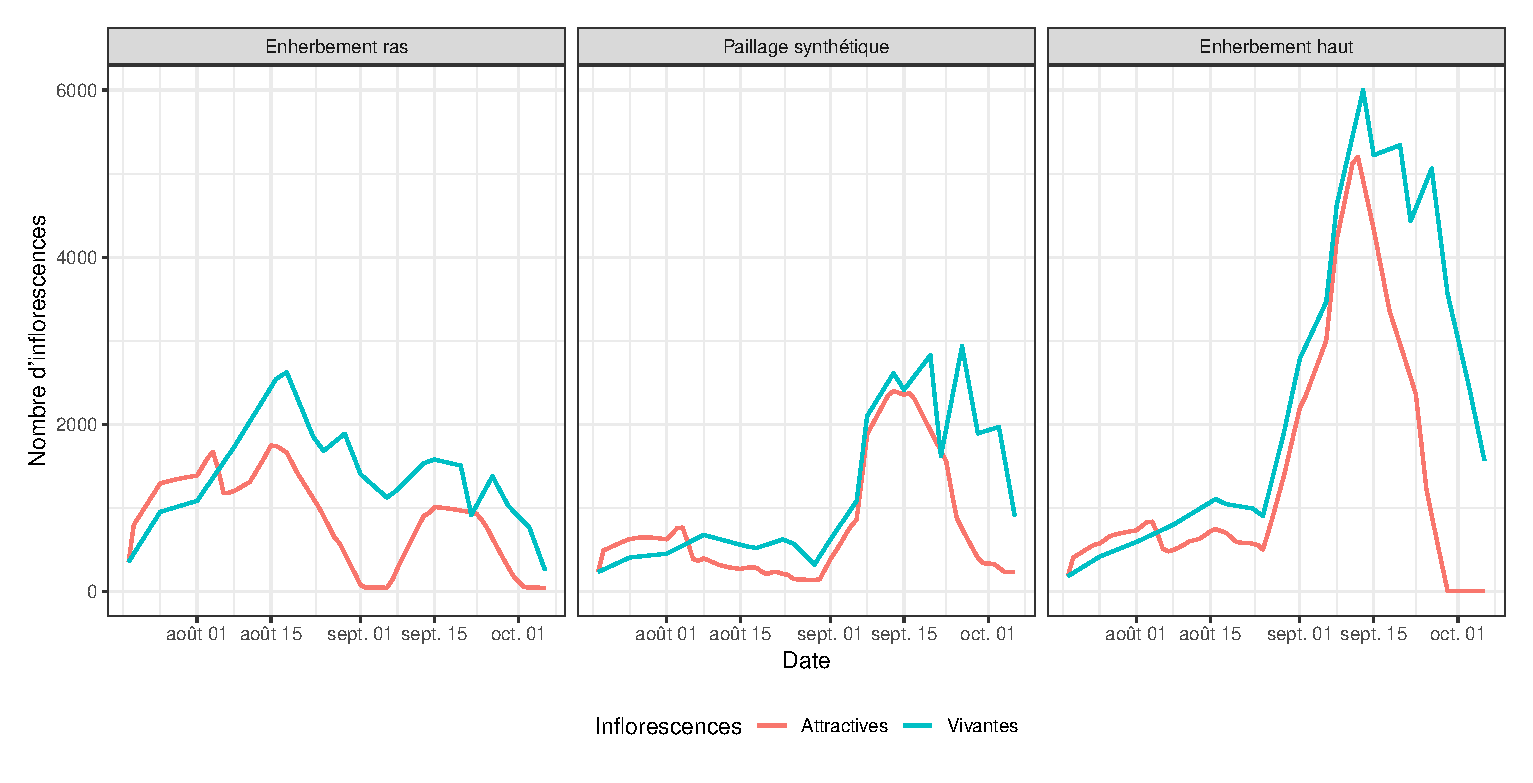
\epsfig{file = plots/inflos_CDE.eps, scale = 0.53}
 \caption{Différence entre les inflorescences vivantes et les inflorescences attractives.}
 \label{fig:CDE}
\end{figure}


Sur les trois solutions--types trouvées après la calibration du modèle, deux correspondent à celles trouvées précédemment.
Les dynamiques sont visibles sur la figure~\ref{fig:C}.
On observe une amélioration sur les sous-parcelles PS et EH, notamment en ce qui concerne la fin de dynamique en fin de saison.
La parcelle ER est en revanche toujours mal captée.
Et la pertinence biologique des solutions (concernant la forte présence ou l'absence d'individus exogènes et l'absence d'individus qui émergents de la sous-parcelle EH) reste toujours discutable.

Les paramètres pour les trois solutions--types sont les suivants :
{%
\newcommand{\mc}[3]{\multicolumn{#1}{#2}{#3}}
\begin{center}
\begin{tabular}{lllllll}
\mc{7}{c}{\textbf{Solution--type 1}}\\
$\gamma$ & $p_{\text{m}}$ & $\mu_{\text{ER}}$ & $\mu_{\text{EH}}$ & $k$ & \texttt{stock} & $E_0\mu_\ell$\\
0.115 & 0.189 & 0.898 & 0.012 & 1.877 & 515 & 3.097\\
 &  &  &  &  &  & \\
\mc{7}{c}{\textbf{Solution--type 2}}\\
$\gamma$ & $p_{\text{m}}$ & $\mu_{\text{ER}}$ & $\mu_{\text{EH}}$ & $k$ & \texttt{stock} & $E_0\mu_\ell$\\
0.004 & 0.490 & 0.990 & 0.018 & 0.242 & 9970 & 5.638\\
 &  &  &  &  &  & \\
\mc{7}{c}{\textbf{Solution--type 3}}\\
$\gamma$ & $p_{\text{m}}$ & $\mu_{\text{ER}}$ & $\mu_{\text{EH}}$ & $k$ & \texttt{stock} & $E_0\mu_\ell$\\
0 & 0.094 & 0.999 & 0.514 & 0.181 & 18214 & 8.259
\end{tabular}
\end{center}
}%


\begin{figure}[ht]
 \centering
 
  \centering
 \textbf{Solution--type 1}
 
 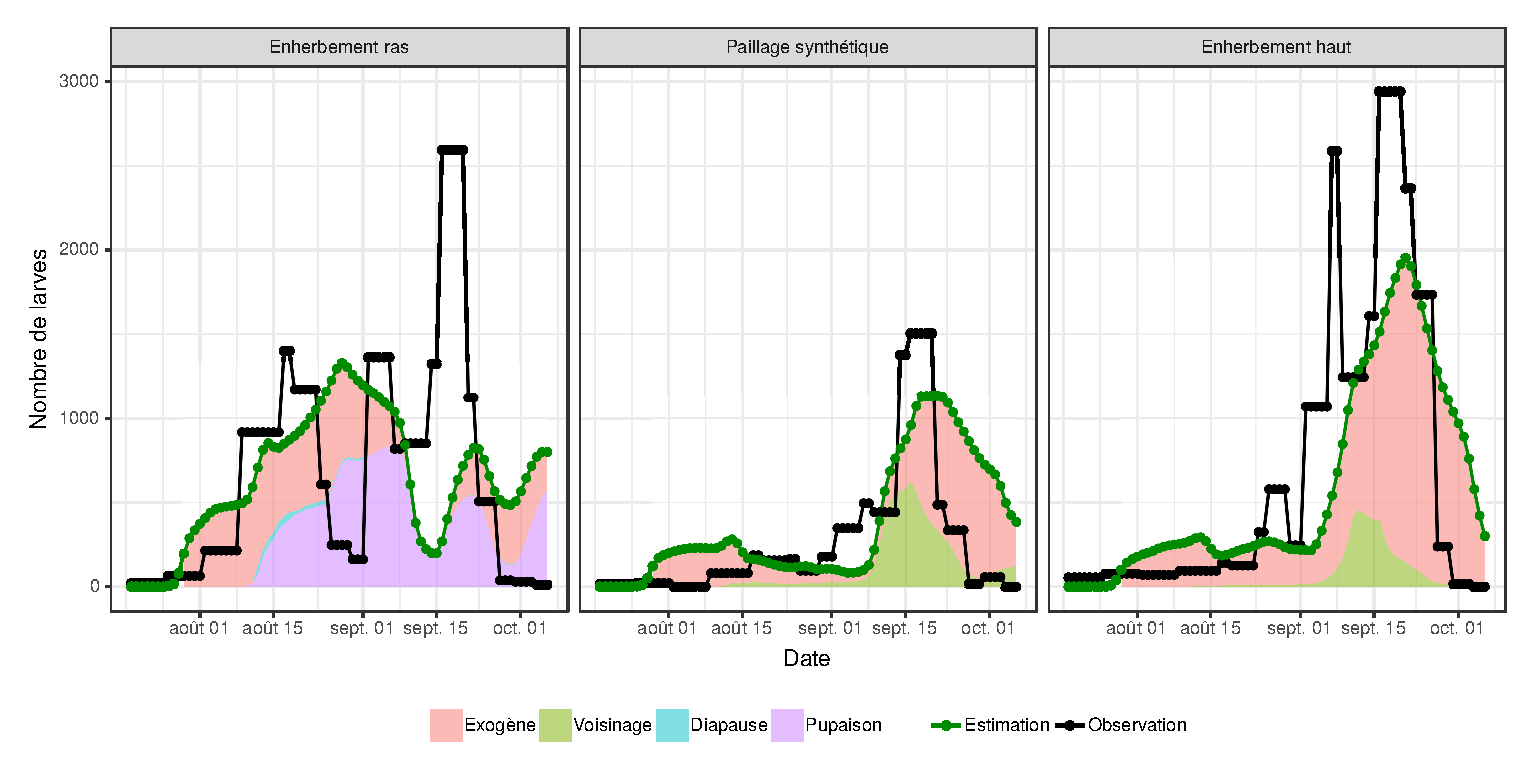
\epsfig{file = plots/C1.eps, scale = 0.52}
 
 \textbf{Solution--type 2}
 
 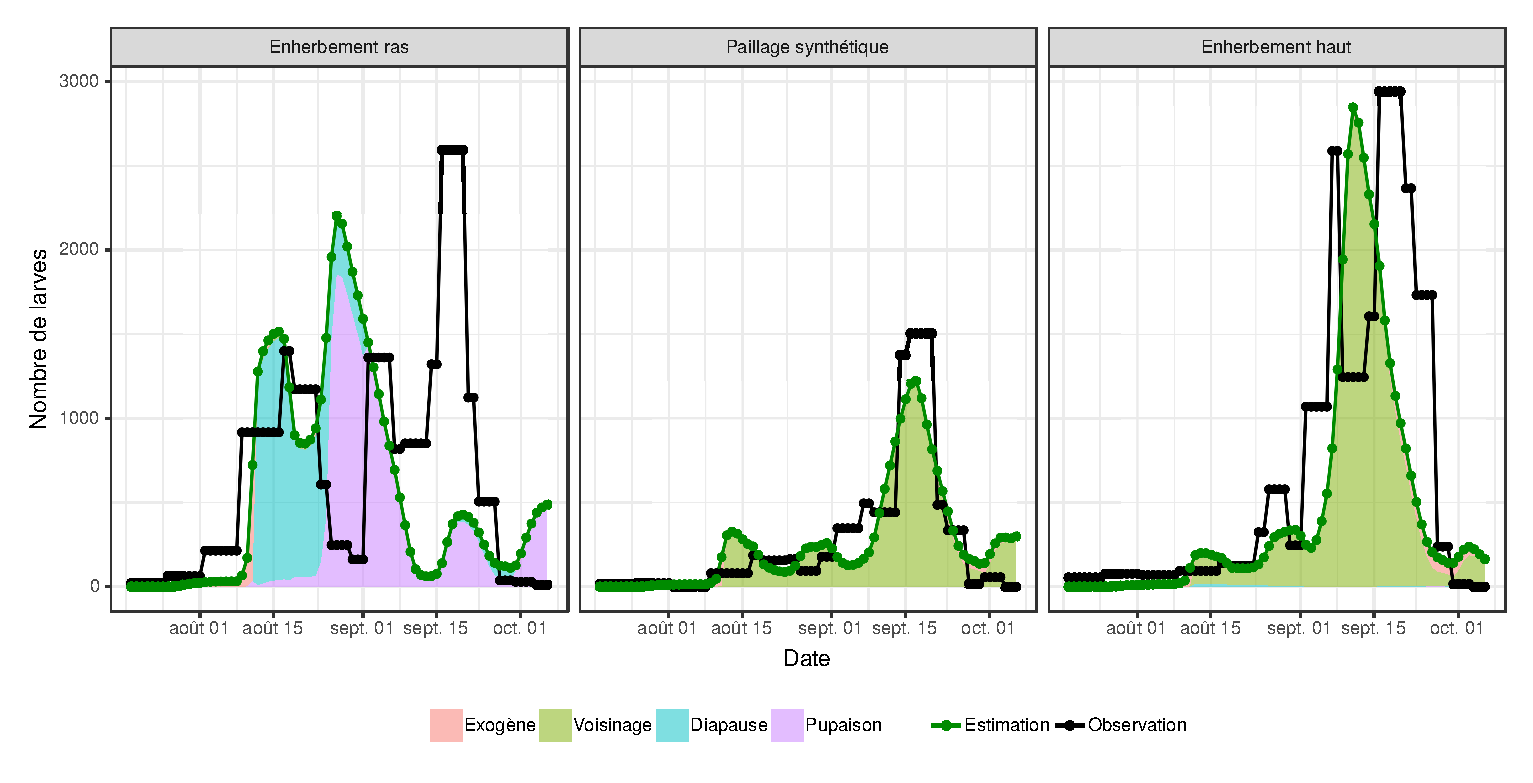
\epsfig{file = plots/C2.eps, scale = 0.52}
 
 \textbf{Solution--type 3}
 
 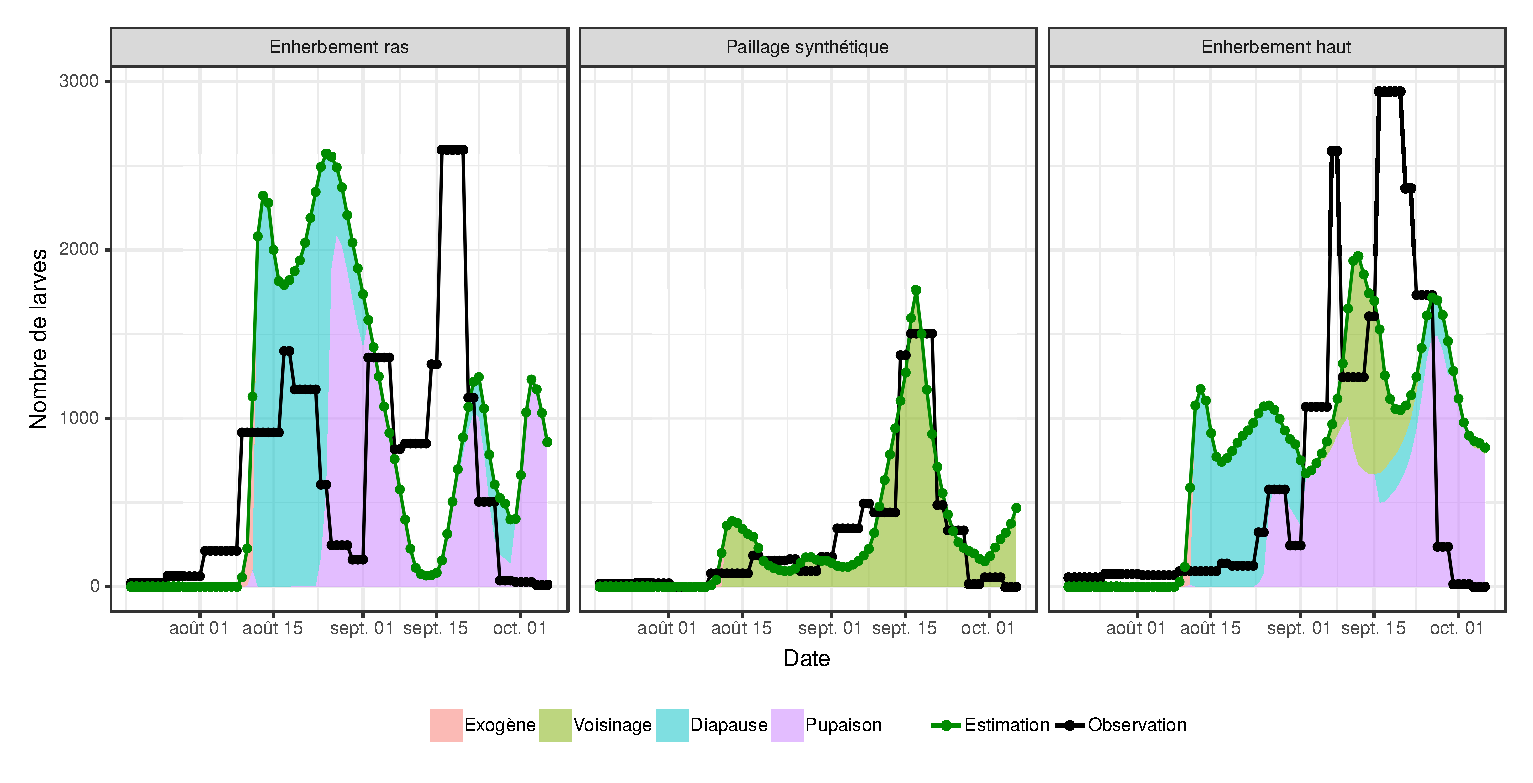
\epsfig{file = plots/C3.eps, scale = 0.52}
 
 
 \caption{Dynamiques observées et simulées pour chacune des trois solutions--types. La décomposition indiquant la provenance des femelles qui ont pondus les œufs est disponible pour les dynamiques simulées.}
 \label{fig:C}
\end{figure}


On remarquera que la prédiction sur la troisième solution--type est toujours aussi mauvaise.
La prise en compte de l'attractivité des inflorescences ne permet toujours pas la baisse des dynamiques observées en fin de saison lorsqu'il y a des individus endogènes dans la sous-parcelle EH.

\clearpage
\section{Solutions avec l'introduction d'un paramètre de saisonnalité}

Les hypothèses émises jusqu'à présent n'ont pas permis d'expliquer ce qu'il se produit en fin de saison.
Aux hypothèses déjà faites, on en rajoute une autre.
Ce que l'on observe sur les dynamiques de larves, c'est qu'il semble y avoir une forte baisse de la population de larves qui s'amorce aux alentours du 15 septembre (sur le verger n\textdegree1).
On émet alors l'hypothèse qu'un phénomène intervient à cette date.
Ce phénomène non-observé caractériserait un changement de la conjoncture sur le verger et induirait une baisse du nombre de larves.

Et on modélise cette hypothèse de manière radicale en introduisant un paramètre de saisonnalité $\xi \in [0;1]$ sur le nombre de femelles dans le verger à partir du 15 septembre.
Cela donne en pratique
\[
F_{t,i} := \begin{cases}
            F_{t, i} & \text{si $t<$ 15 septembre,}\\
            \xi \, F_{t, i} & \text{si $t\geq$ 15 septembre.}
           \end{cases}
\]
Concrètement, si le modèle décide de mettre une valeur éloignée de 1, cela signifie qu'à partir du 15 septembre que le cycle de développement de la cécidomyie subit des perturbations qui entraînent une baisse du nombre de larves produites.

Après calibration du modèle, un scénario se dégage des autres.
Il est visible sur la figure~\ref{fig:D}.
Les paramètres associés sont les suivants :
\begin{center}
\begin{tabular}{llllllll}
$\gamma$ & $p_{\text{m}}$ & $\mu_{\text{ER}}$ & $\mu_{\text{EH}}$ & $k$ & \texttt{stock} & $E_0\mu_{\ell}$ & $\xi$\\
0.021 & 0.105 & 0.938 & 0.916 & 1.992 & 516 & 6.018 & 0.004
\end{tabular}
\end{center}


\begin{figure}[ht]
 \centering
 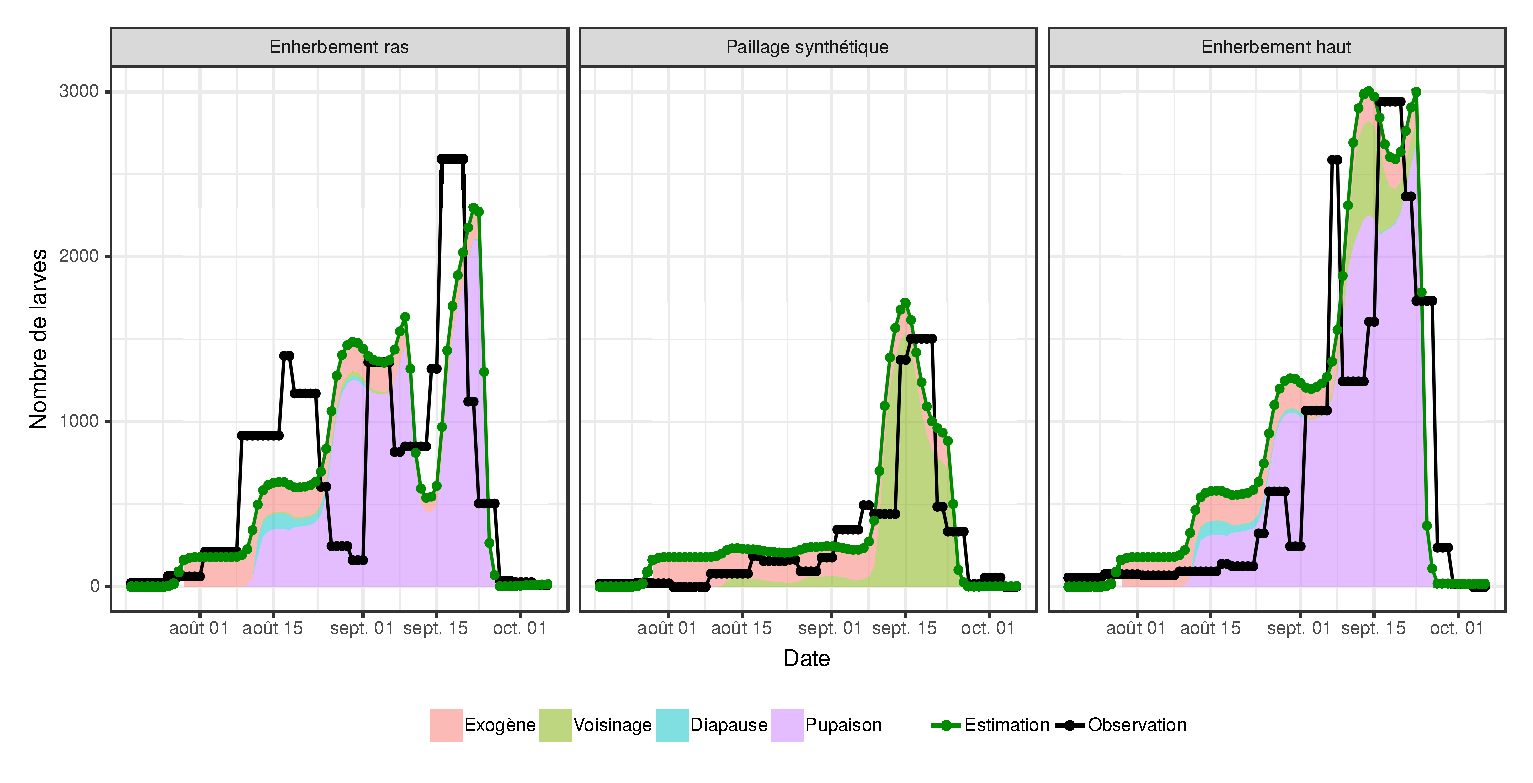
\epsfig{file = plots/D1.eps, scale = 0.59}
 \caption{Dynamiques observées et simulées. La décomposition indiquant la provenance des femelles qui ont pondus les œufs est disponible pour les dynamiques simulées.}
 \label{fig:D}
\end{figure}


Les dynamiques sont ici très bien captées pour les sous-parcelles PS et EH.
La dynamique de la sous-parcelle ER est plutôt bien captée, surtout si l'on relativise vis à vis des des estimations précédentes qui ont toujours étés mauvaises.
Les paramètres montrent (et le graphique aussi) qu'il y a principalement des femelles endogènes, ce qui semble vraisemblable.



Cela semble être une bonne estimation.
On procède à la validation sur le verger n\textdegree2.
Il faut cependant noter que le phénomène de saisonnalité a lieu sur ce verger aux alentours du 23 août pour les modalités PS et EH et aux alentours du 7 septembre pour la modalité ER.

Les résultats produits sur le verger n\textdegree2 sont visibles sur la figure~\ref{fig:D2}.
On remarque que les dynamiques des modalités ER et EH sont plus ou moins captées.
En revanche, si la temporalité de la dynamique de la sous-parcelle PS semble correcte, son intensité n'est pas restituée correctement.
\begin{figure}[ht]
 \centering
 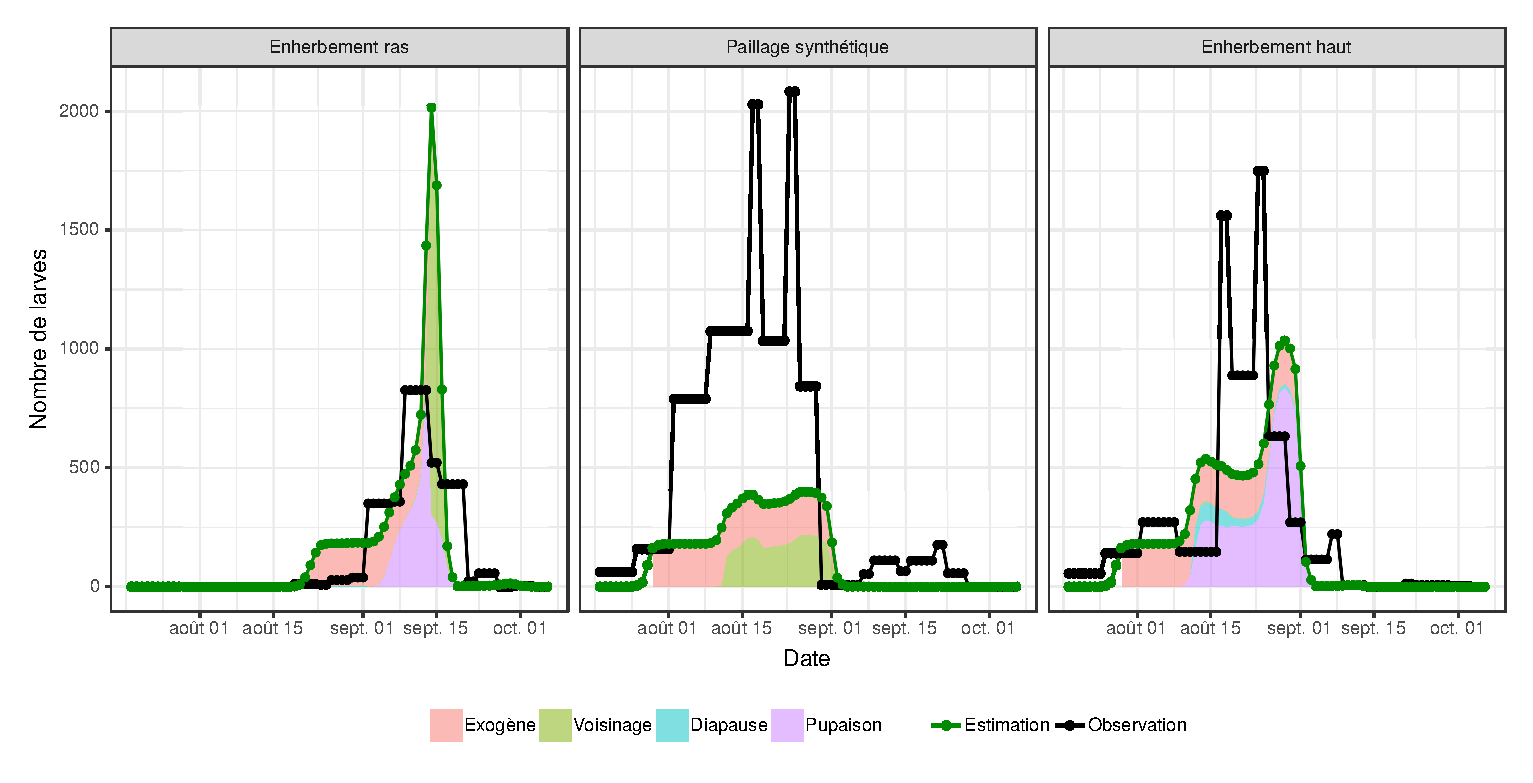
\epsfig{file = plots/D_b2.eps, scale = 0.59}
 \caption{Dynamiques observées et simulées sur le verger n\textdegree2. La décomposition indiquant la provenance des femelles qui ont pondus les œufs est disponible pour les dynamiques simulées.
 Les paramètres utilisés sont ceux calibrés par le modèle sur le verger n\textdegree1.}
 \label{fig:D2}
\end{figure}



% Le fait que les paramètres trouvés par le modèle en calibrant sur le verger n\textdegree1 ne s'applique pas au verger n\textdegree2 peut s'expliquer par la forte variabilité du phénomène observé.
% En effet, si l'une des deux dynamiques observées est très atypiques par rapport au comportement moyen, 








